\documentclass[../main.tex]{subfiles}
\graphicspath{{\subfix{../IMAGES/}}}

\begin{document}
\localtableofcontents

\subsection{Fundamentals}
Four main types : \begin{itemize}
    \item Storage hydropower : uses dam to store water: Two types : \begin{itemize}
        \item Open-loop : at least one reservoir is continuously connected to a naturally flowing water source\\
        \item Closed-loop : no reservoir is connected to a significant natural inflow\\
    \end{itemize}
    \item Pumped storage hydropower : similar to storage hydropower but with pumping capabilities\\
    \item Run-of-river hydropower : flowing water from a river to spin a turbine, provides a continuous supply of electricity\\
    \item Offshore hydropower : tidal currents to generate electricity\\
\end{itemize}
The local mean flow specific energy is given by : \begin{equation}
    h_t = \frac{p}{\rho} + gZ + \frac{C^2}{2} + Cste
\end{equation}

Which gives the available specific energy : \begin{equation}
    E = gH = gH_i - gH_{\overline{i}} = g(Z_B - Z_{\overline{B}}) - \sum gH_r
\end{equation}
With H the head.\\

The hydraulic power is given by : \begin{equation}
    P_h = \rho Q \times E = \rho Q g(H_l - H_{\overline{l}})
\end{equation}

They can be classified by : \begin{table}[hbt!]
    \centering
    \begin{tabular}{p{.28\textwidth}|p{.28\textwidth}|p{.28\textwidth}}
        By types & By head & Power capacity \\ \hline
        Storage, pumped-storage, run of river, offshore & High (>300m), medium (30-300m), low (<30m) & Large (>100MW), medium (25-100MW), small (1-25MW), mini (100kW-1MW), micro (<100kW)
    \end{tabular}
\end{table}

The Net Positive Suction Specific Energy is defined as $NPSE = gH_{\overline{l}} - \frac{p_v}{\rho} - gZ_{ref}$. We need a minimum setting level to avoid cavitation $h_s = Z_{ref} - Z_{\overline{B}} = Z_{\overline{1}} - Z_{\overline{B}}$, with $\overline{1}$ the exit of the turbine, $\overline{l}$ the outlet of the draft tube and $\overline{B}$ the surface of the water.\\
\begin{itemize}
    \item For turbines : $NPSE \simeq g NPSH = \frac{p_a}{\rho} - \frac{p_v}{\rho} - gh_s + \frac{C_{\overline{l}^2}}{2}$ (NPSH : Net Positive Suction Head (m))
    \item For pumps : $NPSE = \frac{p_a}{\rho} - \frac{p_v}{\rho} - gh_s = g NPSH$
    \item Thoma number : $\sigma_{th} = \frac{NPSE}{E}$
\end{itemize}
With $p_a$ the atmospheric pressure and $p_v$ the saturated vapor pressure.

\subsection{Pelton turbines}
Also called impulse turbines. They need high head and low $\nu$.
\begin{itemize}
    \item Head from 300 to 2000m
    \item Unit power up to 420MW
    \item Efficiency up to $92\%$
    \item 1 to 6 injectors
    \item Horizontal or vertical shaft
\end{itemize}

The specific energy balance is given by : $E_t = \frac{C_1^2}{2} - \frac{C_{\overline{1}}^2}{2} + E_{rb}$ ($E_{rb}$ the losses).\\

The absolute flow velocity is then $\overrightarrow{C} = \overrightarrow{U} + \overrightarrow{W}$ with the rotating velocity $\overrightarrow{U} = \omega \times X = \omega R$ and the relative flow velocity $\overrightarrow{W} = \overrightarrow{C} - \overrightarrow{U}$.\\

Assume no specific energy losses between bucket inlet and outlet : $W_1^2 = W_{\overline{1}}^2$ and $\Vec{W}_{\overline{1}} \Vec{U}_{\overline{1}} = -U_{\overline{1}} W_{\overline{1}} \cos \beta_{\overline{1}}$.\\
$E_t = W_1 U_1 + \cos \beta_{\overline{1}} U_1 -E_{rb} $\\

\begin{itemize}
    \item Maximum specific energy ($\beta_{\overline{1}} = 0, U_1= \frac{C_1}{2}$) : $E_t^{max} = \frac{C_1^2}{2}-E_{rb}$
    \item Maximum power $P^{max} = \rho \frac{\pi D_2^2}{4} \frac{C_1^3}{2}$
\end{itemize}

Needle stroke : \begin{itemize}
    \item Energy balance : $E = \frac{C_2^2}{2} + \sum_i E_{r_i}$, $\sum_i E_{r_i} = E e_r$ the $\%$ specific energy lost in the nozzle.
    \item Discharge : $Q = z_0 A_2 C_2 = z_0 \frac{\pi D_2^2}{4}C_2 = z_0 \frac{\pi D_2^2}{4} \sqrt{2E(1-e_r)}$
    \item Power : $P = z_0 \rho \frac{\pi D_2^2}{4} \frac{(2E(1-e_r))^{3/2}}{2}$
\end{itemize}
With $z_0$ the number of injectors.\\

Jet specific speed : \begin{itemize}
    \item Jet discharge : $\frac{Q}{z_0} = \frac{\pi D_2^2}{4} \sqrt{(1-e_r) 2E}$
    \item Specific speed : $\nu_0 = \frac{\pi}{60} (1-e_r)^{1/4} \frac{ND_2}{\sqrt{2E}}$
    \item Optimum speed : $U_1 = \frac{C_2}{2}\Leftrightarrow \frac{\pi}{30} N \frac{D_1}{2} = \frac{\sqrt{2E(1-e_r)}}{2}$
\end{itemize}

\begin{figure}[hbt!]
    \centering
    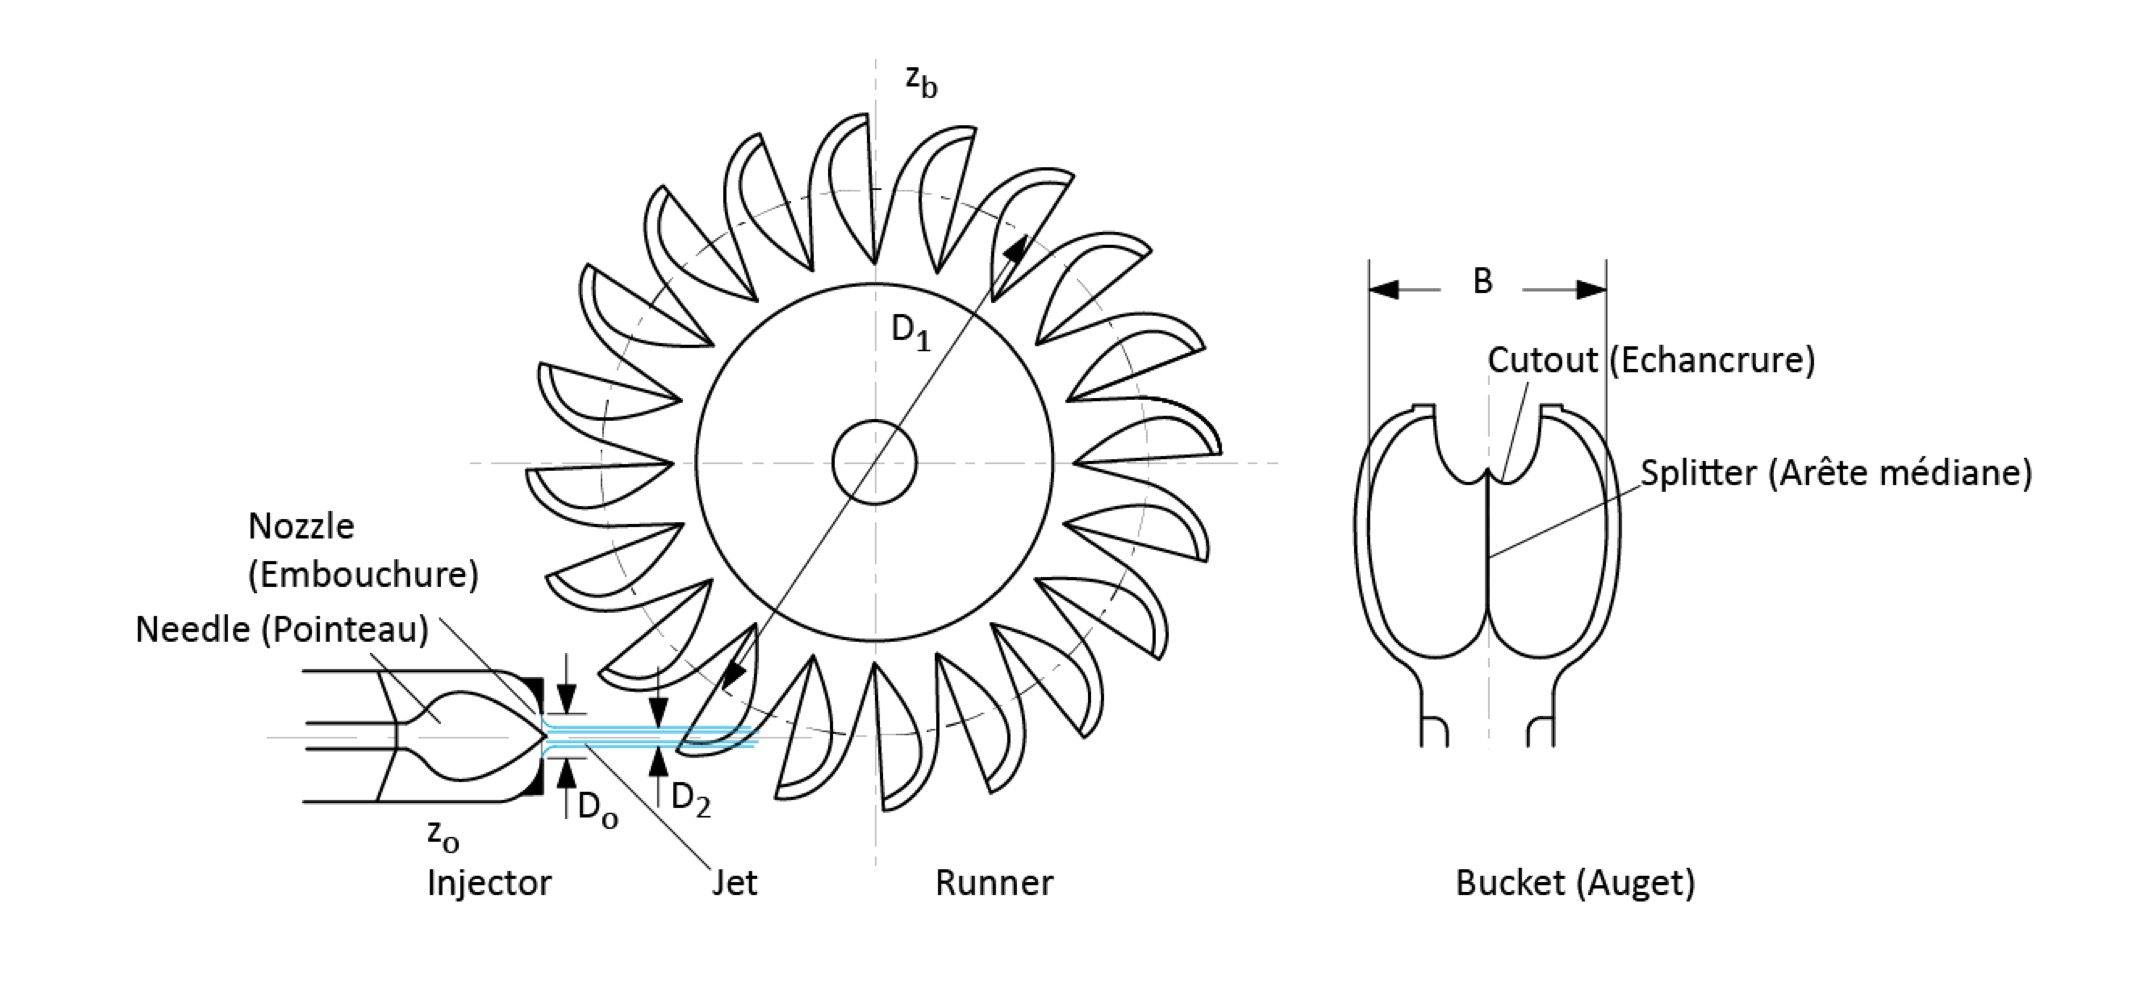
\includegraphics[width=0.8\linewidth]{IMAGES/Hydraulic/IMG_0186.jpeg}
\end{figure}
The jet diameter ($D_2$) is linked to the bucket's width ($B_2$) by : $D_2 \simeq \frac{B_2}{3/3.4}$.\\
Let $D_1$ be the diameter of the runner at the center of the buckets. We have $\nu_0 = \frac{(1-e_r)^{3/4}}{2} \frac{D_2}{D_1}$.\\
The flow coefficient can also give an insight on the design of the turbine as $\psi_1 = \frac{3.6}{1-0.735 \frac{B_2}{D_1}}$.\\

The pelton turbine are affected by silt erosion. Buckets need to be coated. Another issue is the dynamic loading; buckets are subject to vibration, centrifugal stress and jet deviation ($\sigma_m$ : mean stress, $\sigma_a$ : dynamic stress < 30MPa in general, then $R = \frac{\sigma_{min}}{\sigma_{max}} = \frac{\sigma_m - \sigma_a}{\sigma_m + \sigma_a}$)\\

\subsection{Reaction turbines}
Different kinds : Francis, Kaplan and Bulb turbines.\\

\subsubsection{Francis runners}
Flow is radial. Suited for medium head. \\
We first have some stay vanes (non movable) and then the guide vanes (movable). The more the guide vanes are opened, the higher the discharge will be.

\begin{figure}[hbt!]
    \centering
    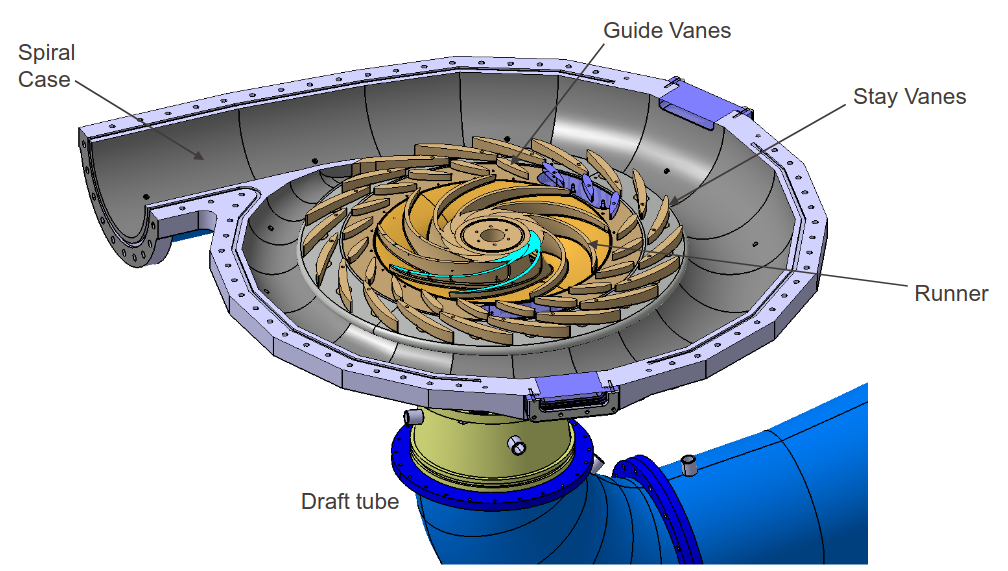
\includegraphics[width=0.6\linewidth]{IMAGES/Hydraulic/Screenshot from 2024-10-16 14-26-05.png}
\end{figure}

The extracted energy at the external radius is then (Euler's equation) : \begin{equation}
    E_t = C_{1e} U_{1e} - \frac{1}{2}C_{\overline{1e}} U_{\overline{1e}}
\end{equation}

For partial load ($Q<Q_{BEP})$, we can get precession vortex rope. Above the best efficiency point we get axisymmetric vortex rope. \\
The issues are therefore : \begin{itemize}
    \item Noise, vibration
    \item Cavitation erosion
    \item Operation instability
    \item Performance alteration (efficiency, characteristic curves)
\end{itemize}

\subsubsection{Kaplan turbines}
Axial flow, low head.\\
Bulb turbines are fully axial or mixed flow (the generator is submerged) whereas Kaplan ones are more like Francis turbines.\\
The inlet and outlet diameter are the same : $A_1 = \pi \frac{D_{1e}^2 - D_{1i}^2}{4}$.\\

Kaplan runners have controllable pitch. \\

Because we have two degree of freedom, the efficiency curve is in 3D. For every parameter, it forms an on-com curve such that for a given Power, we can find the best discharge, guide vane opening angle and kaplan's angle. \\

Main issues : \begin{itemize}
    \item Erosion risk (leading edge cavitation, tip vortex, discharge ring erosion, guide vane wakes-blades interactions)
    \item Efficiency alteration (hub cavitation, wear and tear)
\end{itemize}

\subsection{Pumping units}
Reasons for pumped storage power stations : \begin{itemize}
    \item Electrical energy cannot be directly stored
    \item Matching the demand of energy
    \item Seasonal, daily energy balance
    \item Services to the grid
\end{itemize}

Types of pumped-storage power plant : \begin{itemize}
    \item Binary group : unit equipped with reversible pump-turbines
    \item Ternary group : turbine and pump on the same shaft
    \item Quaternary group : separated pumping and generating units
\end{itemize}

\subsubsection{Binary group}
Mostly Francis-type reversible pump-turbine.\\
In generating mode, we have $gH_1 - g H_{\overline{1}} = g(Z_B - Z_{\overline{B}}) - \sum g H_r$\\
In pumping mode, we have $gH_1 - g H_{\overline{1}} = g(Z_B - Z_{\overline{B}}) + \sum g H_r$. The flow is axial at the inlet : $Cu_{\overline{1}} = 0$ and at the outlet $Cu_1 = \frac{U_1}{2}$. We then have that : \begin{itemize}
    \item $Q_{opt} = \frac{1}{2} U_1 A_1 \tan \beta_1$
    \item $E_{t,max} = \frac{U_1^2}{2} $
    \item $Cu_{1,opt} = \frac{U_1}{2}$
    \item $P_{opt} = \rho A_1 \tan \beta_1 \frac{U_1^3}{4}$
\end{itemize}

Extended operating range allows for compensation of head variations and allow the avoidance of cavitation. 


\quad \underline{Hydraulic by-pass :}\\
We use both pumping and generating at the same time to reduce costs of pumping. $P_{tot} = P_g + P_p$.\\

Advantages of reversible pump-turbines : \begin{itemize}
    \item Fixed speed : compact, low investments costs
    \item With additional variable speed : efficient power control in pumping mode, comply with large head variations, extended operating range in turbine and pumping mode, fast active power injection
\end{itemize}

Disadvantages : \begin{itemize}
    \item Fixed speed : hydraulic design (trade-off between pumping and generating mode leads to lower efficiency), operating range restricted due to flow instability in partial load, long start-up time and switch off operating mode
    \item With additional variable speed : investment costs for the electromechanical equipment, specific power limited for a given rotational speed
\end{itemize}

\subsubsection{Ternary group}
Three machines : electrical machine, hydraulic turbine and pump. They are classified based on the shaft orientation.\\
Usually Pelton + pump (multistage). Matching both pumping and generating modes. High grade control. One direction of rotation. Safe transients.\\

Advantages : \begin{itemize}
    \item High operational flexibility
    \item Easy and short time start-up in pump mode
    \item Adjustable pump power with hydraulic by-pass
    \item Wide operating range with Pelton turbines
    \item Increased efficiency in pump and turbine modes
    \item Smooth hydraulic transients
\end{itemize}

Disadvantages : \begin{itemize}
    \item High investment costs
    \item Maintenance costs due to electromechanical complexity and number of components
    \item Increased ventilation losses in pumping mode
    \item Lower efficiency in case of hydraulic by-pass
    \item Instability risks for the rotating train for vertical units
\end{itemize}

\subsubsection{Quaternary group}
Four machines : two electrical machines, a turbine and a pump. \\

Advantages : \begin{itemize}
    \item Optimization for efficiency 
    \item Fastest responding pumped hydro technology
\end{itemize}

Disadvantages : \begin{itemize}
    \item Space requirements for hosting 2 power houses
    \item Investment costs and maintenance
\end{itemize}

\subsection{Sustainability for hydropower}
Sustainability definition origin as a tri-dimensional concept (economy, social, ecology). \\

\begin{figure}[hbt!]
    \centering
    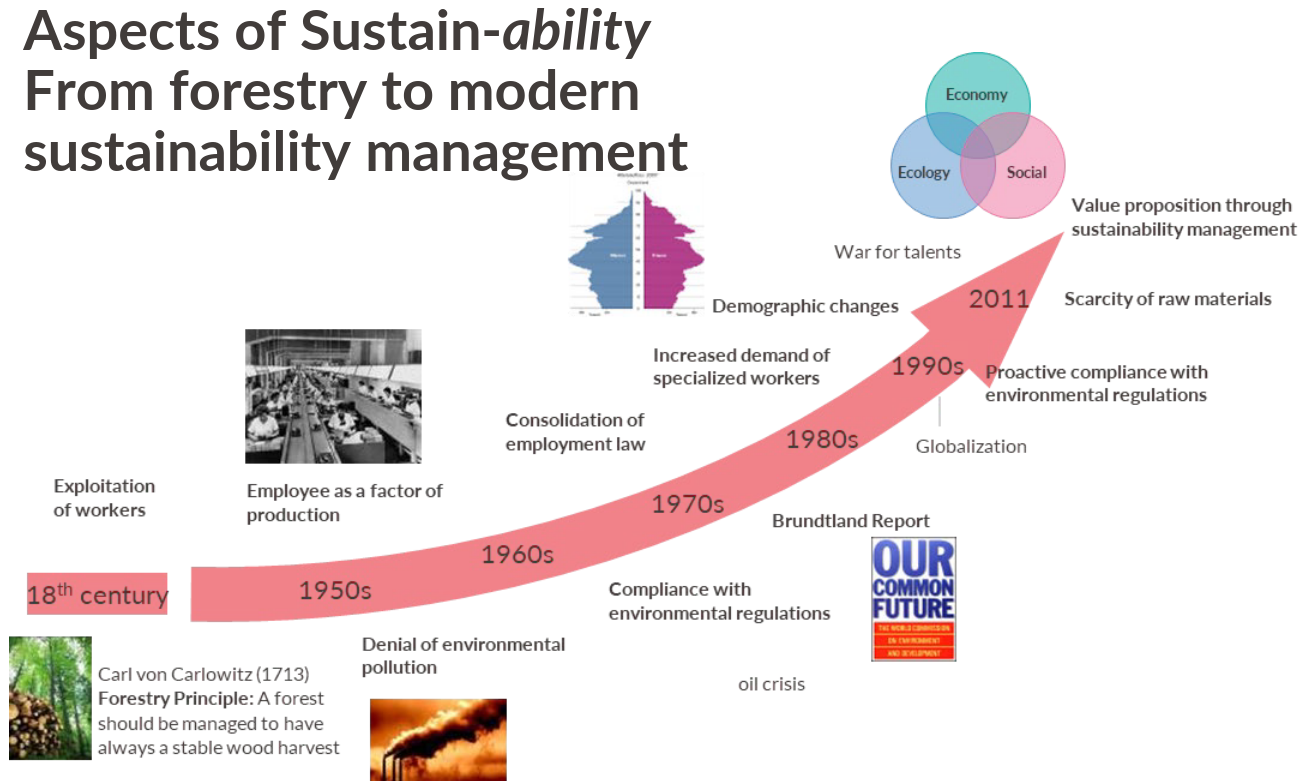
\includegraphics[width=0.8\linewidth]{IMAGES/Hydraulic/Screenshot from 2024-11-20 14-23-43.png}
\end{figure}

Value of contribution of sustainability create value, take opportunities, manage risks : \begin{itemize}
    \item creating value : new technologies, new products for now requirements.
    \item cost savings : reduction in the electricity, natural gas, fuels and water consumption. Water reduction
    \item strengthening of market position : avoidance of reputational risks, increase the attractiveness for employees.
\end{itemize}
Organizations' sustainability action areas and corresponding goals need to be defined, reported and published under the consideration of essentiality.\\

Sustainability pillars of hydropower : \begin{itemize}
    \item Economical
    \item Societal
    \item Environmental
\end{itemize}

\begin{itemize}
    \item Resilient infrastructure : projects demonstrate their ability to respond to the effects of climate change, it takes into account regional water needs and availability
    \item Good governance : projects are governed by sound corporate business structures, treat their workers fairly and respectfully
    \item Health ecosystem : projects contribute to restore ecosystems and invest in forest, river and other ecosystem conservation and restoration. Projects manages impacts to ecosystems, such as erosion, and sedimentation.
    \item Prosperous communities : projects engage in good faith with affected communities. Project share their benefits with affected communities. Societal acceptance and positive impacts on local communities are part of sustainability evaluation of projects.
\end{itemize}
\warning A project's location determines the limits of achievable usefulness and sustainability.\\

\begin{figure}[hbt!]
    \centering
    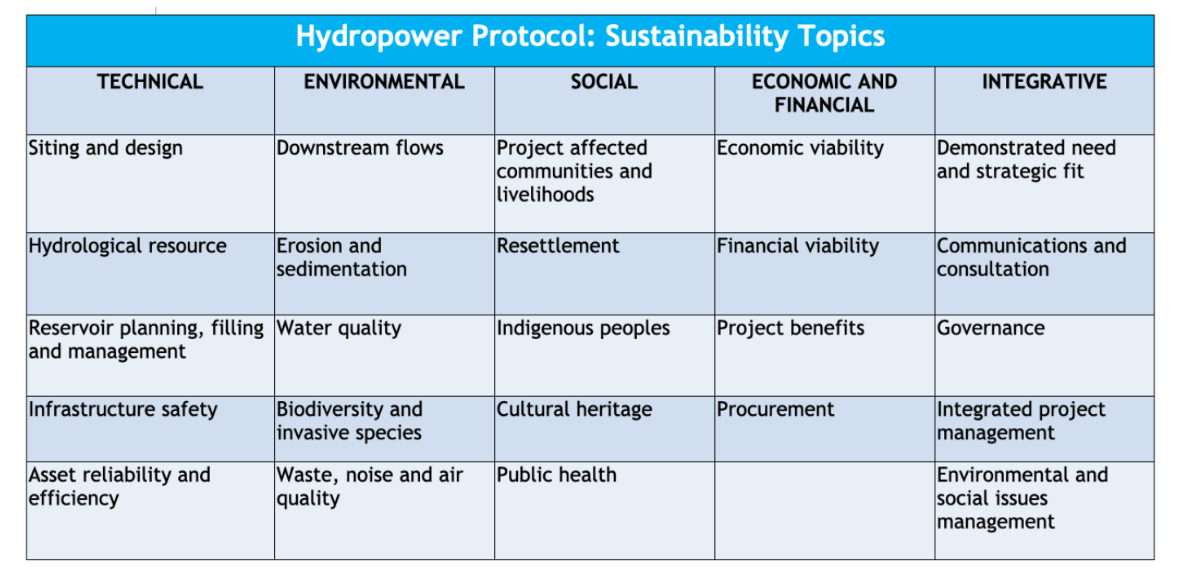
\includegraphics[width=0.7\linewidth]{IMAGES/Hydraulic/Screenshot from 2024-11-20 15-43-25.png}
    \caption{Protocol for hydropower sustainability standards}
\end{figure}



\end{document}